\subsubsection*{\underline{\textsc{\Large Imp}}}
\noindent\emph{Tiny Fiend (Devil), Lawful Evil}

\noindent\rule{0.5\textwidth}{0.5pt}

\noindent\textbf{Armor Class}: 13

\noindent\textbf{Hit Points}: 10 (3d4 + 3)

\noindent\textbf{Speed}: 20 ft., fly 40 ft.

\noindent\rule{0.5\textwidth}{0.5pt}
\begin{table}[H]
	\begin{tabular}{cccccc}
		\textbf{STR} & \textbf{DEX} & \textbf{CON} & \textbf{INT} & \textbf{WIS} & \textbf{CHA} \\
		6 (-2) & 17 (+3) & 13 (+1) & 11 (+0) & 12 (+1) & 14 (+2) \\
	\end{tabular}
\end{table}
\noindent\rule{0.5\textwidth}{0.5pt}

\noindent\textbf{Skills}: Deception +4, Insight +3, Persuasion +4, Stealth +5

\noindent\textbf{Damage Resistances}:  Cold; Bludgeoning, Piercing, and Slashing from Nonmagical Attacks that aren't Silvered

\noindent\textbf{Damage Immunities}: Fire, Poison

\noindent\textbf{Condition Immunities}: Poisoned

\noindent\textbf{Senses}: darkvision 120 ft., Passive Perception 11

\noindent\textbf{Languages}: Common, Infernal

\noindent\textbf{Challenge}: 1 (200 XP)

\noindent\rule{0.5\textwidth}{0.5pt}

\noindent\textbf{Shapechanger}: The imp can use its action to polymorph into a beast form that resembles a rat (speed 20 ft.), a raven (20 ft., fly 60 ft.), or a spider (20 ft., climb 20 ft.), or back into its true form. Its statistics are the same in each form, except for the speed changes noted. Any equipment it is wearing or carrying isn't transformed. It reverts to its true form if it dies.

\noindent\textbf{Devil's Sight}: Magical darkness doesn't impede the imp's darkvision.

\noindent\textbf{Magic Resistance}: The imp has advantage on saving throws against spells and other magical effects.

\noindent\rule{0.5\textwidth}{0.5pt}

\noindent\textbf{ACTIONS}

\noindent\textbf{Sting (Bite in Beast Form)}: Melee Weapon Attack: +5 to hit, reach 5 ft., one target. Hit: 5 (1d4 + 3) piercing damage, and the target must make a DC 11 Constitution saving throw, taking 10 (3d6) poison damage on a failed save, or half as much damage on a successful one.

\noindent\textbf{Invisibility}: The imp magically turns invisible until it attacks or until its concentration ends (as if concentrating on a spell). Any equipment the imp wears or carries is invisible with it.

\begin{center}
	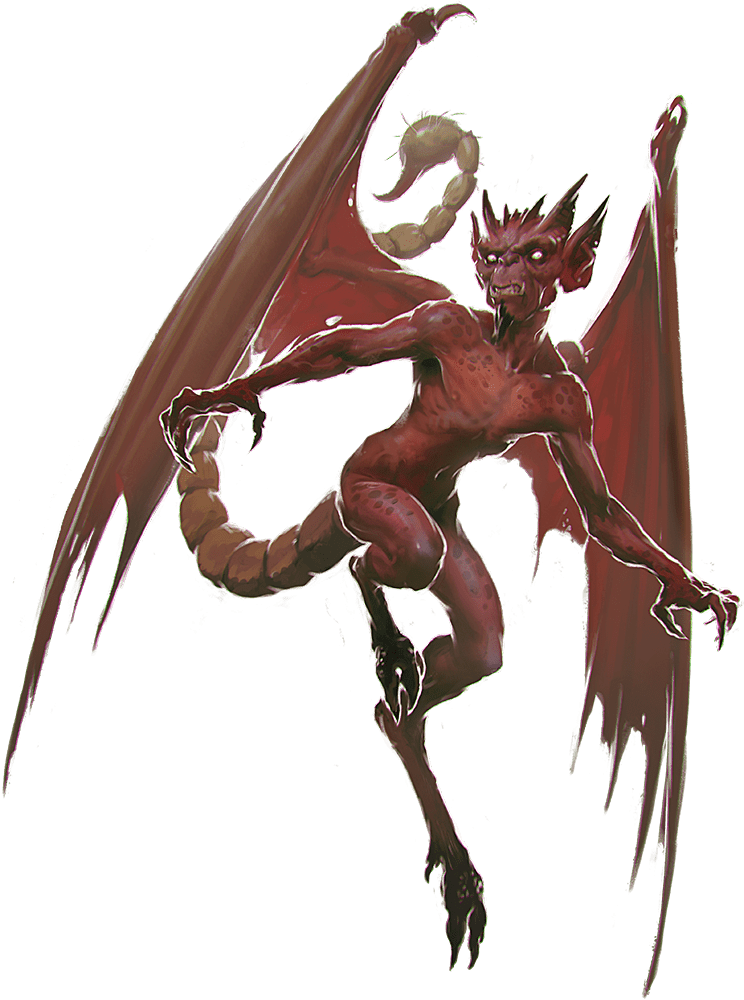
\includegraphics[width = 0.3\textwidth]{imp}
	
	\emph{Imp}
\end{center}